\begin{figure}[htbp]
\centering
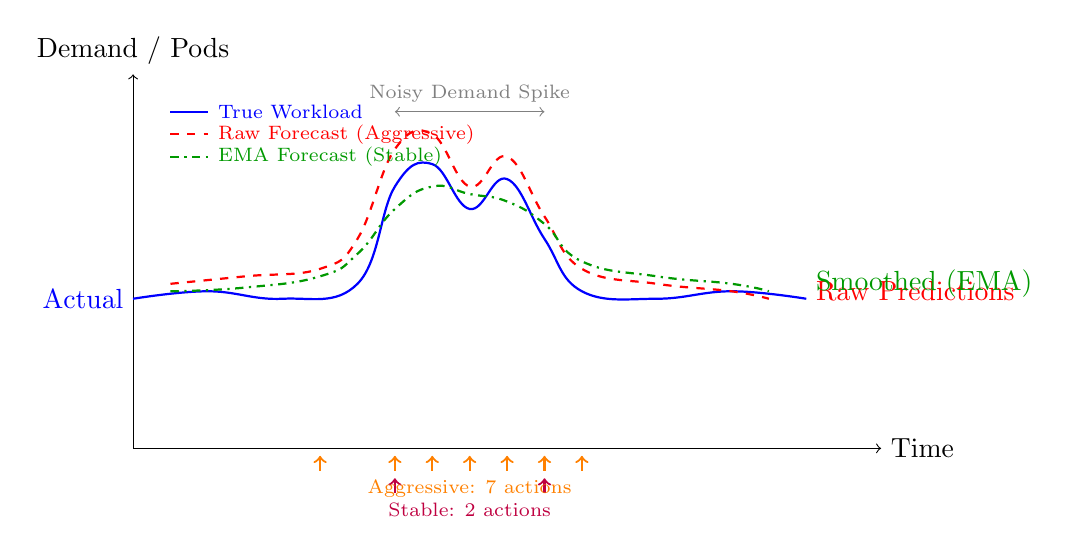
\begin{tikzpicture}[scale=0.95]

% Axes
\draw[->] (0,0) -- (10,0) node[right] {Time};
\draw[->] (0,0) -- (0,5) node[above] {Demand / Pods};

% True workload - noisy spike
\draw[thick, blue] plot[smooth, tension=0.7] coordinates {
  (0,2) (1,2.1) (2,2) (3,2.2) (3.5,3.5) (4,3.8) (4.5,3.2) (5,3.6) (5.5,2.8) (6,2.1) (7,2) (8,2.1) (9,2)
};

% ML predictions - following spike with noise
\draw[thick, red, dashed] plot[smooth, tension=0.7] coordinates {
  (0.5,2.2) (1.5,2.3) (2.5,2.4) (3,2.8) (3.5,4.0) (4,4.2) (4.5,3.5) (5,3.9) (5.5,3.1) (6,2.4) (7,2.2) (8,2.1) (8.5,2.0)
};

% Smoothed predictions - less volatile
\draw[thick, green!60!black, dashdotted] plot[smooth, tension=0.8] coordinates {
  (0.5,2.1) (1.5,2.15) (2.5,2.3) (3,2.6) (3.5,3.2) (4,3.5) (4.5,3.4) (5,3.3) (5.5,3.0) (6,2.5) (7,2.3) (8,2.2) (8.5,2.1)
};

% Aggressive PAKS scaling actions (frequent)
\foreach \x in {2.5, 3.5, 4.0, 4.5, 5.0, 5.5, 6.0} {
  \draw[thick, orange, ->] (\x, -0.3) -- (\x, -0.1);
}

% Stability-Aware PAKS scaling actions (sparse)
\foreach \x in {3.5, 5.5} {
  \draw[thick, purple, ->] (\x, -0.6) -- (\x, -0.4);
}

% Labels
\node[blue, left] at (0, 2) {Actual};
\node[red, right] at (9, 2.1) {Raw Predictions};
\node[green!60!black, right] at (9, 2.2) {Smoothed (EMA)};

% Scaling event labels
\node[orange, below, font=\scriptsize] at (4.5, -0.3) {Aggressive: 7 actions};
\node[purple, below, font=\scriptsize] at (4.5, -0.6) {Stable: 2 actions};

% Spike annotation
\draw[<->, gray] (3.5, 4.5) -- (5.5, 4.5) node[midway, above, font=\scriptsize] {Noisy Demand Spike};

% Legend
\draw[thick, blue] (0.5, 4.5) -- (1.0, 4.5) node[right, font=\scriptsize] {True Workload};
\draw[thick, red, dashed] (0.5, 4.2) -- (1.0, 4.2) node[right, font=\scriptsize] {Raw Forecast (Aggressive)};
\draw[thick, green!60!black, dashdotted] (0.5, 3.9) -- (1.0, 3.9) node[right, font=\scriptsize] {EMA Forecast (Stable)};

\end{tikzpicture}
\caption{Conceptual comparison of Aggressive PAKS vs. Stability-Aware PAKS response to a noisy demand spike. Raw predictions closely track high-frequency fluctuations, triggering frequent scaling actions (orange arrows). Exponential smoothing filters transient noise, resulting in fewer, more deliberate scaling decisions (purple arrows). Hysteresis and cooldown further suppress action unless sustained change is detected.}
\label{fig:controller_comparison}
\end{figure}
